% Options for packages loaded elsewhere
\PassOptionsToPackage{unicode}{hyperref}
\PassOptionsToPackage{hyphens}{url}
\PassOptionsToPackage{dvipsnames,svgnames,x11names}{xcolor}
%
\documentclass[
  super,
  preprint,
  3p]{elsarticle}

\usepackage{amsmath,amssymb}
\usepackage{iftex}
\ifPDFTeX
  \usepackage[T1]{fontenc}
  \usepackage[utf8]{inputenc}
  \usepackage{textcomp} % provide euro and other symbols
\else % if luatex or xetex
  \usepackage{unicode-math}
  \defaultfontfeatures{Scale=MatchLowercase}
  \defaultfontfeatures[\rmfamily]{Ligatures=TeX,Scale=1}
\fi
\usepackage{lmodern}
\ifPDFTeX\else  
    % xetex/luatex font selection
\fi
% Use upquote if available, for straight quotes in verbatim environments
\IfFileExists{upquote.sty}{\usepackage{upquote}}{}
\IfFileExists{microtype.sty}{% use microtype if available
  \usepackage[]{microtype}
  \UseMicrotypeSet[protrusion]{basicmath} % disable protrusion for tt fonts
}{}
\makeatletter
\@ifundefined{KOMAClassName}{% if non-KOMA class
  \IfFileExists{parskip.sty}{%
    \usepackage{parskip}
  }{% else
    \setlength{\parindent}{0pt}
    \setlength{\parskip}{6pt plus 2pt minus 1pt}}
}{% if KOMA class
  \KOMAoptions{parskip=half}}
\makeatother
\usepackage{xcolor}
\setlength{\emergencystretch}{3em} % prevent overfull lines
\setcounter{secnumdepth}{5}
% Make \paragraph and \subparagraph free-standing
\ifx\paragraph\undefined\else
  \let\oldparagraph\paragraph
  \renewcommand{\paragraph}[1]{\oldparagraph{#1}\mbox{}}
\fi
\ifx\subparagraph\undefined\else
  \let\oldsubparagraph\subparagraph
  \renewcommand{\subparagraph}[1]{\oldsubparagraph{#1}\mbox{}}
\fi


\providecommand{\tightlist}{%
  \setlength{\itemsep}{0pt}\setlength{\parskip}{0pt}}\usepackage{longtable,booktabs,array}
\usepackage{calc} % for calculating minipage widths
% Correct order of tables after \paragraph or \subparagraph
\usepackage{etoolbox}
\makeatletter
\patchcmd\longtable{\par}{\if@noskipsec\mbox{}\fi\par}{}{}
\makeatother
% Allow footnotes in longtable head/foot
\IfFileExists{footnotehyper.sty}{\usepackage{footnotehyper}}{\usepackage{footnote}}
\makesavenoteenv{longtable}
\usepackage{graphicx}
\makeatletter
\def\maxwidth{\ifdim\Gin@nat@width>\linewidth\linewidth\else\Gin@nat@width\fi}
\def\maxheight{\ifdim\Gin@nat@height>\textheight\textheight\else\Gin@nat@height\fi}
\makeatother
% Scale images if necessary, so that they will not overflow the page
% margins by default, and it is still possible to overwrite the defaults
% using explicit options in \includegraphics[width, height, ...]{}
\setkeys{Gin}{width=\maxwidth,height=\maxheight,keepaspectratio}
% Set default figure placement to htbp
\makeatletter
\def\fps@figure{htbp}
\makeatother

\makeatletter
\makeatother
\makeatletter
\makeatother
\makeatletter
\@ifpackageloaded{caption}{}{\usepackage{caption}}
\AtBeginDocument{%
\ifdefined\contentsname
  \renewcommand*\contentsname{Table of contents}
\else
  \newcommand\contentsname{Table of contents}
\fi
\ifdefined\listfigurename
  \renewcommand*\listfigurename{List of Figures}
\else
  \newcommand\listfigurename{List of Figures}
\fi
\ifdefined\listtablename
  \renewcommand*\listtablename{List of Tables}
\else
  \newcommand\listtablename{List of Tables}
\fi
\ifdefined\figurename
  \renewcommand*\figurename{Figure}
\else
  \newcommand\figurename{Figure}
\fi
\ifdefined\tablename
  \renewcommand*\tablename{Table}
\else
  \newcommand\tablename{Table}
\fi
}
\@ifpackageloaded{float}{}{\usepackage{float}}
\floatstyle{ruled}
\@ifundefined{c@chapter}{\newfloat{codelisting}{h}{lop}}{\newfloat{codelisting}{h}{lop}[chapter]}
\floatname{codelisting}{Listing}
\newcommand*\listoflistings{\listof{codelisting}{List of Listings}}
\makeatother
\makeatletter
\@ifpackageloaded{caption}{}{\usepackage{caption}}
\@ifpackageloaded{subcaption}{}{\usepackage{subcaption}}
\makeatother
\makeatletter
\@ifpackageloaded{tcolorbox}{}{\usepackage[skins,breakable]{tcolorbox}}
\makeatother
\makeatletter
\@ifundefined{shadecolor}{\definecolor{shadecolor}{rgb}{.97, .97, .97}}
\makeatother
\makeatletter
\makeatother
\makeatletter
\makeatother
\journal{Journal Name}
\ifLuaTeX
  \usepackage{selnolig}  % disable illegal ligatures
\fi
\usepackage[]{natbib}
\bibliographystyle{elsarticle-num}
\IfFileExists{bookmark.sty}{\usepackage{bookmark}}{\usepackage{hyperref}}
\IfFileExists{xurl.sty}{\usepackage{xurl}}{} % add URL line breaks if available
\urlstyle{same} % disable monospaced font for URLs
\hypersetup{
  pdftitle={CRUSE to Safe Cycling in Ireland},
  pdfauthor={Robin Lovelace; Joey Talbot; Eugeni Vidal Tortosa; Hussein Mahfouz; Elaine Brick; Peter Wright; Gary O'Tool; Dan Brennan; Suzanne Meade},
  pdfkeywords={Cycling, Open-source, Road Safety, Active Travel},
  colorlinks=true,
  linkcolor={blue},
  filecolor={Maroon},
  citecolor={Blue},
  urlcolor={Blue},
  pdfcreator={LaTeX via pandoc}}

\setlength{\parindent}{6pt}
\begin{document}

\begin{frontmatter}
\title{CRUSE to Safe Cycling in Ireland \\\large{An Open Source
Methodology to Support Active Travel} }
\author[1]{Robin Lovelace%
\corref{cor1}%
}
 \ead{r.lovelace@leeds.ac.uk} 
\author[1]{Joey Talbot%
%
}

\author[1]{Eugeni Vidal Tortosa%
%
}

\author[1]{Hussein Mahfouz%
%
}

\author[2]{Elaine Brick%
%
}

\author[3]{Peter Wright%
%
}

\author[2]{Gary O'Tool%
%
}

\author[4]{Dan Brennan%
%
}

\author[4]{Suzanne Meade%
%
}


\affiliation[1]{organization={University of
Leeds},addressline={Institute for Transport Studies, Leeds, LS2 9JT,
United Kingdom},postcodesep={}}
\affiliation[2]{organization={AECOM},addressline={Unit 6, Galway
Technology Park, Parkmore, Galway, Ireland},postcodesep={}}
\affiliation[3]{organization={AECOM},addressline={Winslade House,
Winslade Park, Manor Drive, Clyst St Mary, EXETER, EX5 1FY,
UK},postcodesep={}}
\affiliation[4]{organization={Transport Infrastructure
Ireland},addressline={Parkgate Business Centre, Parkgate Street, Dublin
8, D08 DK10, Ireland},postcodesep={}}

\cortext[cor1]{Corresponding author}









        
\begin{abstract}
Under the EU Road infrastructure safety management (RISM) directive, the
National Road Safety Strategy (RSS), and the Climate Action Plan
Transport Infrastructure Ireland (TII) has a remit for road safety and
decarbonizing a predominantly road-based network in Ireland.

To address data needs for both safety and project evaluation on the
National Road Network (NRN), the Cycle Route Uptake and Scenario
Estimation (CRUSE) Tool was developed. While cycling in Ireland
represents only 3\% of total modal share, with higher intensities in
urban areas, the levels of cycling collisions are disproportionately
high at 20\% of all serious injuries and 7\% of all fatalities. If
Ireland is to meet its climate and safety targets, data to establish
baseline cycling levels and future cycling levels is needed.

Due to an absence of reliable data, particularly rural cycling levels,
TII commissioned the Institute for Transport Studies (ITS) at the
University of Leeds and AECOM to develop a new tool for this purpose.
ITS Leeds led the development of the PCT for England and Wales, which
has ``revolutionized the practice of strategic cycle planning
nationally''. The tool is an open-source approach using recognized
open-source methodology to enable planners, engineers, and other
stakeholders to make evidence-based decisions for the NRN. CRUSE is
available at \url{https://cruse.bike/} and builds on the Propensity to
Cycle Tool (PCT) for England and Wales. CRUSE goes beyond the PCT in
several important ways, higher resolution data, more trip types,
including estimates for education, inter-urban, and recreational trips.
In addition to understanding cycling intensity, for asset planning and
management purposes, the tool provides essential road safety information
to enable reporting of disaggregate collision rates.

CRUSE is structured in a similar way to the traditional four-stage
transport model, but its use of Open Street Map (OSM) data, used by
\href{https://www.cyclestreets.net/}{Cyclestreets.net} for routing,
enables network quality to be assessed without costly surveys to record
new infrastructure. OSM tags generate ``cycle friendliness'' estimates
of all links on the network, based on existing recorded infrastructure.
A range of networks is provided, highlighting routes for directness
(Fastest) and ``cycle friendliness'' (Quietest). It uses origin and
destination data from the 2016 Census in combination with modeled demand
data to estimate cycling levels and potential at the area, route, and
network levels for each county in Ireland and offers estimates of the
baseline level of cycling and several future scenario-based levels of
cycling.

As countries, like Ireland, invest in cycling, the number of killed and
seriously injured cyclists must reduce too. The CRUSE Tool provides
estimates of cycling potential and routing for each county in Ireland,
and works in both urban and rural settings, to enable monitoring of
cycling safety. With growth in the E-bike market, the tool will help
inform inter-urban and rural networks to support the transfer of trips
to sustainable modes for longer journeys. The CRUSE Tool methodology and
findings are directly relevant to addressing the challenges and
opportunities faced by other NRAs. The datasets resulting from the
project are open access and can be used by both non-experts and
professionals.
\end{abstract}





\begin{keyword}
    Cycling \sep Open-source \sep Road Safety \sep 
    Active Travel
\end{keyword}
\end{frontmatter}
    \ifdefined\Shaded\renewenvironment{Shaded}{\begin{tcolorbox}[frame hidden, boxrule=0pt, interior hidden, sharp corners, borderline west={3pt}{0pt}{shadecolor}, enhanced, breakable]}{\end{tcolorbox}}\fi

\newpage{}

\hypertarget{introduction}{%
\section{Introduction}\label{introduction}}

Mobility kills. High energy transport systems are a major contributor to
climate change, a leading cause of premature death and injury due to
road traffic collisions, and a cause of disease due to airborne
pollutants. Conversely, evidence-based and effective transport
\emph{policies} have great potential to decarbonize economies, improve
public health, and save lives.

Transport is responsible for 23\% of global emissions, 70\% of which is
from road transport, nearly half of which (around 10\% of global
emissions) is from passenger cars \citep{jaramillo2022}. The transport
system encourages, enables and in some cases enforces unsustainable
lifestyles, including over-consumption of goods due to excessive mobile
storage space and dependency on services that are only accessible by car
due to land use plans that have built up around roads
\citep{gray2001, shergold2012, motte-baumvol2010}.

Recognizing the growing evidence of such impacts of poorly designed and
performing transport systems, governments in many countries have set
targets and taken actions. In the context of climate, road safety and
physicial inactivity crises, policies to improve transport systems can
be classified according to the `Avoid-Shift-Improve' (ASI) framework
\citep{jaramillo2022}. The framework highlights the importance of demand
reduction (\emph{avoid}ing unnecessary trips), in addition to mode
\emph{shift} and \emph{improvement} of existing energy converters, in
that order.

Uptake of cycling, the main topic of this paper, should be seen in this
broader context of transport decarbonisation \citep{brand2020} and
sustainable mobility \citep{burns2013}. Although cycling uptake appears
on the surface to only relate to the `shift' part of the ASI framework,
closer consideration of the knock-on impacts of cycling uptake shows
that it can also help avoid unnecessary trips \citep{nello-deakin2020}.
The rapid uptake of highly efficient e-bikes can also be seen as an
improvement on most electric vehicles, which are too heavy and expensive
to be a sustainable alternative and could in fact delay the transition
away from car dependency and inadvertently enable ``high travel
lock-in'' \citep{anable2019}. At the European level, the European Union
has a target of reducing greenhouse gas emissions by 55\% by 2030,
compared to 1990 levels, and to achieve `net-zero' by 2050.{[}\^{}1{]}

Regarding road traffic casualties, another deadly consequence of
inefficient transport systems, the Road Infrastructure Safety Management
(RISM) directive (2008/96/EC) requires member states to implement a road
safety management system (RSMS) for all public roads. Specifically,
``Member States shall ensure that the ranking of high accident
concentration sections and the network safety ranking are carried
out''.\footnote{https://eur-lex.europa.eu/legal-content/EN/TXT/?u
  ri=celex\%3A32008L0096} Given that `safety' in this context is
usefully quantified as the number of people killed and seriously injured
(KSI) per distance travelled, the directive requires estimation of
distance travelled by mode, down to the road link level. For active
modes, about which there is a paucity of data compared with motorized
modes, this is a major challenge. Better data to inform road safety
policies and interventions is a motivation for the CRUSE tool outlined
in this paper, and modeling active travel more broadly.

In Ireland, the Road Safety Authority (RSA) has set the target of
halving the number of road traffic deaths and serious injuries by
2030.{[}\^{}3{]} Doing so while simultaneously enabling rapid uptake of
active modes will require key active travel routes to be identified and
improved.

A proactive approach to the development of cycling policy and
infrastructure is taking place in Ireland. The main framework
underpinning these efforts is the Climate Action Plan\footnote{\url{https://www.gov.ie/en/publication/7bd8c-climate-action-plan-2023/}}
and The National Development Plan\footnote{\url{https://www.gov.ie/en/publication/774e2-national-development-plan-2021-2030/}}
. Strategic alignment is also outlined by the Phoenix Park Transport and
Mobility Options Study, which highlights public support for active
travel interventions: ``83\% of respondents supported enhanced walking
and cycling facilities'' .

At the regional level, the recently published Greater Dublin Area
Transport Strategy\footnote{\url{https://www.nationaltransport.ie/planning-and-investment/strategic-planning/greater-dublin-area-transport-strategy/}}
reinforces these findings: ``nearly a quarter of adults cycle at least
once a week in the Dublin Metropolitan Area'' with cycling in the Dublin
area taking up to 60,000 cars off the road today. Extrapolating this on
a per population basis across Ireland, with around 40\% of the
population living in Dublin, this suggests that around 150,000 cars
could be removed nationwide just by achieving Dublin levels of cycling
in all counties (notwithstanding existing cycling trips and differences
in trip distances).

Further evidence of the importance of cycling in Ireland \emph{already}
is provided by the National Strategic Objective (NSO) from the National
Development Plan, with €8.6 billion allocated to sustainable transport
infrastructure including public transport and active travel
interventions. Cycle infrastructure will be developed in synchrony with
the BusConnects project, an entire redesign of the bus network in Dublin
and Cork.

It was in this context that Transport Infrastructure Ireland (TII)
commissioned the Cycle Route Uptake and Scenario Estimation (CRUSE)
project. Based on the Propensity to Cycle Tool (PCT) for England and
Wales, the CRUSE tool was developed to provide evidence on current
cycling levels and future cycling potential nationwide across Ireland. A
key consideration for TII is to ensure both urban and rural Ireland were
targeted for cycling infrastructure, as shown in
Figure~\ref{fig-dublin}. To this end, TII extensively reviewed activity
on Irish Roads and how the road network was being used by commuters,
cyclists, heavy goods vehicles and other road users across the Irish
transport network. The aim was for the tool to provide strong, national,
systematic but locally-specific evidence to monitor cycling friendliness
and safety in Ireland, to ensure strategic alignment with national,
regional and local policies. The open source and publicly available
nature of the tool ensures more inclusive and evidence-based
conversations around cycle network planning between all stakeholders in
the transport planning process. Other use cases in the Irish context
includes monitoring the need for existing cycling infrastructure
upgrades, undertaking appraisal, as well as safety and exposure
information in line with the European Cycling Federation, Dutch Cycling
Embassy recommendations and the European RISM Directive, for reporting
collision rates of vulnerable road users by 2024. These factors mean
that the tool can be seen as an open access `leverage point' in the
planning system \citep{lovelace2020}.

\begin{figure}

{\centering 

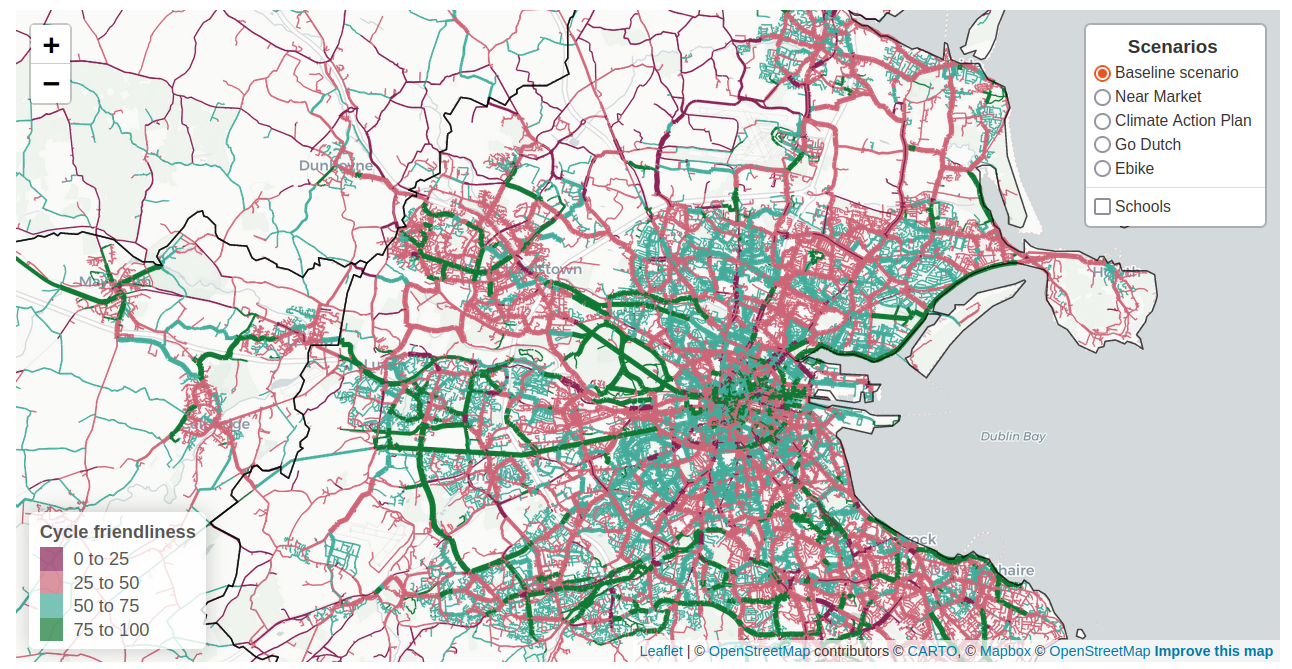
\includegraphics{images/paste-1.png}

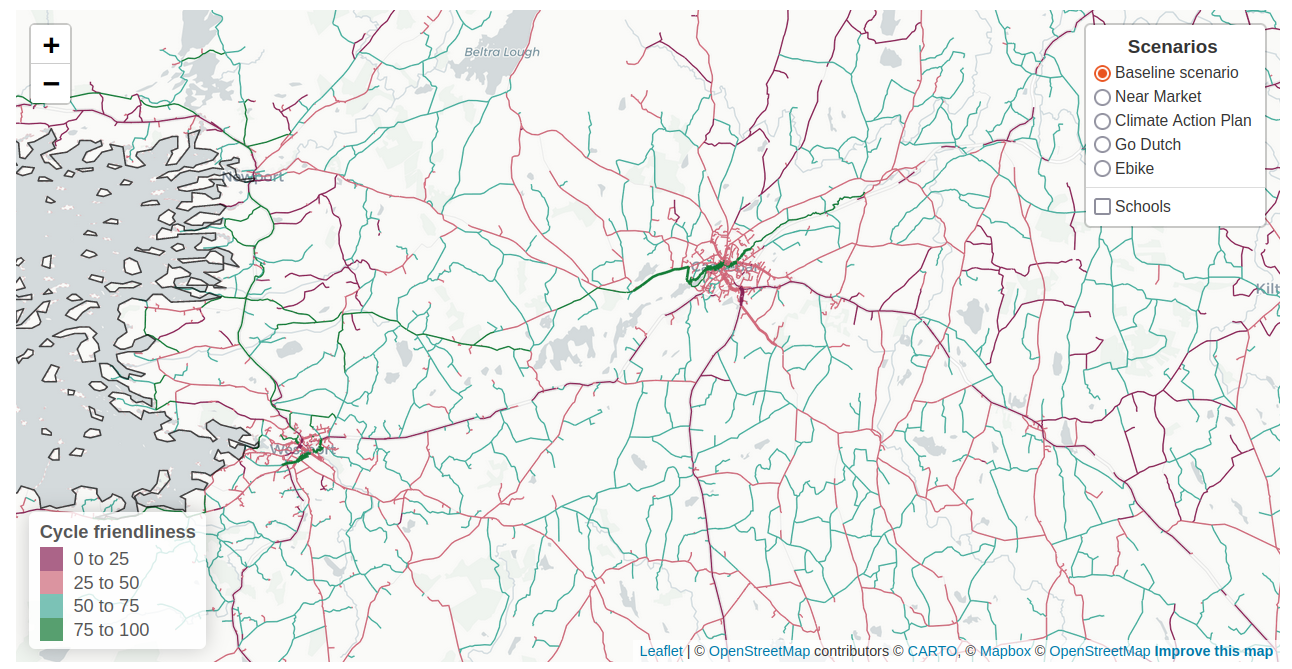
\includegraphics{images/paste-3.png}

}

\caption{\label{fig-dublin}Illustration of the density of route networks
generated by the CRUSE tool for Dublin City and surroundings (top) and
rural County Mayo on the West coast of Ireland. Source: CRUSE tool,
available at \url{https://cruse.bike/}.}

\end{figure}

The rest of paper is structured as follows. In
Section~\ref{sec-methods}, we outline the methods used to generate the
evidence presented in the CRUSE tool for Ireland. In
Section~\ref{sec-results}, we present the results of the CRUSE tool,
including estimates of current cycling levels and future cycling
potential at the national, regional and local levels. In
Section~\ref{sec-discussion}, we discuss the implications of the results
for policy and practice. In Section~\ref{sec-conclusions}, we conclude
the paper.

\hypertarget{sec-methods}{%
\section{Methods and data}\label{sec-methods}}

The methods used to generate the evidence presented in the CRUSE tool
for Ireland build on the Propensity to Cycle Tool (PCT), which was
originally funded by the UK's Department for Transport and developed by
a multi-university team. An important feature of the PCT is that it is
open source and publicly available (at
\href{https://www.pct.bike/}{www.pct.bike}), allowing its use by all
stakeholders in the transport planning process \citep{lovelace2017}. The
PCT approach has had major policy impacts, as outlined in Research
Excellence Framework (REF) impact case studies, which demonstrate that
the tool ``revolutionised strategic cycle planning in England and
Wales''\footnote{See REF Impact Case Study ``Cycle network policy,
  planning and investment transformed by the Propensity to Cycle Tool''
  at
  \href{https://results2021.ref.ac.uk/impact/847d1191-7f25-46ba-a399-b481125edc8f}{results2021.ref.ac.uk}
  submitted by the University of Leeds.} by overcoming the barriers to
cycling investment imposed by lack of evidence on cycling
potential\footnote{See the REF Impact Case Study ``Creating Step Changes
  in Cycling Policy and Infrastructure Planning across the UK'' at
  \href{https://results2021.ref.ac.uk/impact/4BBF3436-FD10-4C75-9791-F5E98AB4411B}{results2021.ref.ac.uk}
  submitted by the University of Westminster.}.

The first version of the PCT was based on current and future potential
uptake of cycling for single stage \emph{travel to work} at desire line,
zone, route, and route network levels \citep{lovelace2016}. It was
launched in April 2017 as the government-endorsed tool for strategic
cycle network planning, as part of the Cycling and Walking Investment
Strategy \citep{cycling2017}. Extensions of the PCT approach have
included estimation of benefits at the individual level
\citep{woodcock2018}, addition of travel to school network
\citep{goodman2019}, and improved modelling of impacts on health,
environmental and distributional outcomes \citep{woodcock2021}.
Initially developed just for England, the PCT was extended to cover all
of Wales (for commuter data only) in 2018.

The PCT approach has been applied in other countries, including Ireland
(the topic of this paper), Scotland, and Portugal. In Portugal the
`biclaR' project, based on methods underlying the PCT, has been
developed and deployed for the Lisbon metro region. The resulting
evidence is available in an interactive web application hosted at
\href{https://biclar.tmlmobilidade.pt}{biclar.tmlmobilidade.pt}
\citep{felix2023}. biclaR includes estimates of impacts, using the World
Health Organisation (WHO) `HEAT for Cycling' tool\footnote{See the
  Health economic assessment tool for walking and cycling at
  \href{https://www.heatwalkingcycling.org/\#homepage}{www.heatwalkingcycling.org}.}
and an `intermodality' scenario that combines cycling with currently
available public transit options based on General Transit Feed
Specification (GTFS) data.

The CRUSE tool seeks to overcome the following methodological
limitations of the original PCT:

\begin{itemize}
\tightlist
\item
  Low resolution of data, with routes starting and ending in
  administrative zone centroids
\item
  Limited coverage of trip purposes beyond travel to work and school
\item
  A web interface that was not user-friendly or intuitive
\end{itemize}

Methods were developed to overcome each of these, as outlined in
Section~\ref{sec-trip-purposes} to Section~\ref{sec-ui}.

\hypertarget{sec-disaggregation}{%
\subsection{Disaggregation of origin-destination
data}\label{sec-disaggregation}}

A feature of active travel interventions is that they require dense
networks of routes to be effective \citep{parkin2018}. This means that
high levels of geographic resolution are needed in the data used to
estimate cycling potential. However, datasets on travel patterns are
often only available at the level of administrative zones. The Central
Statistics Office (CSO) in Ireland provides Place of Work, School or
College Census of Anonymised Records
(\href{https://www.cso.ie/en/census/census2016reports/powscar/}{POWSCAR})
data on the number of people travelling to work and school at the
Electoral Division (ED) level, for example.

The method used to convert OD data to route networks used in the PCT was
to calculate a single route between the population weighted centroids
associated with each OD pair. This method works fine when the OD data
represents movement between small areas, but was not appropriate for
generating route networks from the POWSCAR data because zone centroids
are so far apart that the resulting route networks would be sparse and
unrealistic. To tackle this issue we developed a new method for OD data
disaggregation called `jittering' \citep{lovelace2022}. The method works
by first disaggregating the OD data based on a `disaggregation
threshold' and then assigning each disaggregated `sub-OD' pair to
`subpoints' within each zone. As shown in Figure~\ref{fig-dublin}, the
resulting route networks are dense, even in rural areas.

\hypertarget{sec-trip-purposes}{%
\subsection{Additional trip purposes}\label{sec-trip-purposes}}

A limitation of the original PCT was that it only included travel to
work data. This was partially addressed by the inclusion of travel to
school based on data from the Department for Education in England
\citep{goodman2019}. An advantage of the POWSCAR OD data over OD
datasets derived from census surveys in many countries is that it
includes travel to school data. We commissioned a version of POWSCAR
that included a breakdown of the total flows between OD pairs by purpose
and mode, enabling a more realistic estimation of the `Baseline' cycling
network.

However, travel to school and work only constitute a small proportion of
all trips. To overcome this issue, we developed a spatial interaction
modelling methodology to estimate the number of trips between each OD
pair for additional trip purposes.

The classification of trip purposes used in the CRUSE tool was guided
mainly by the trip purpose classification found within the National
Household Travel Survey (NHTS), but with the addition of categories
based on the comprehensive POWSCAR data, and the need to include
recreational trips and multi-stage trips (not yet implemented). An
overview of the trip purposes used in CRUSE is presented in
Figure~\ref{fig-trip-purposes}.

\begin{figure}

{\centering 

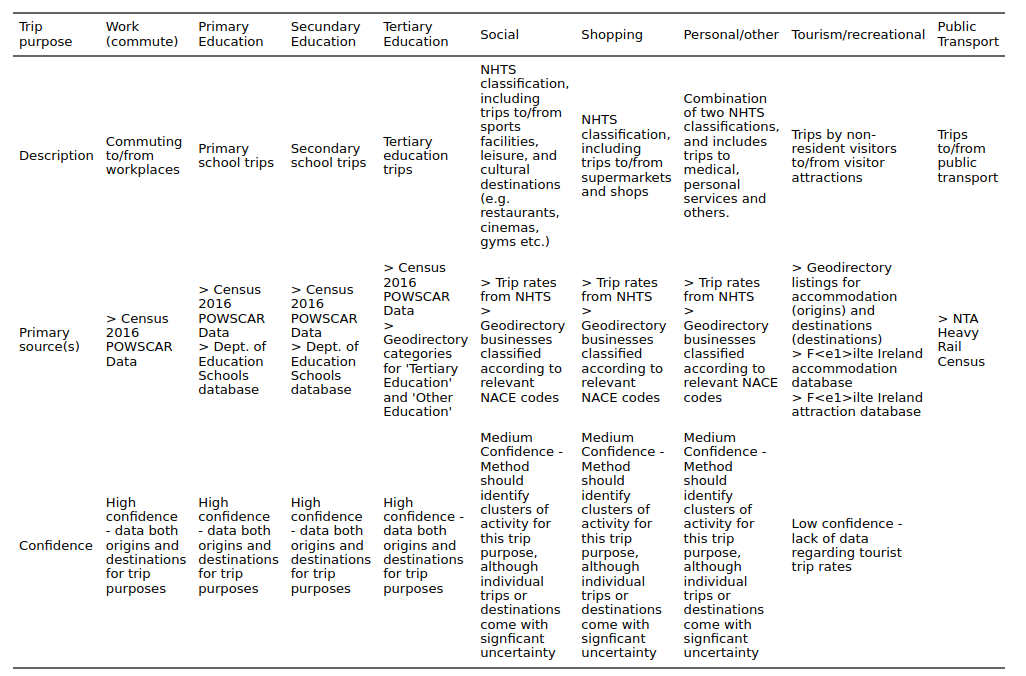
\includegraphics{images/paste-4.png}

}

\caption{\label{fig-trip-purposes}Trip purposes used in the CRUSE tool.}

\end{figure}

\hypertarget{sec-ui}{%
\subsection{User interface}\label{sec-ui}}

\hypertarget{sec-results}{%
\section{Results}\label{sec-results}}

National planning

Regional

Local

\hypertarget{sec-discussion}{%
\section{Discussion}\label{sec-discussion}}

\hypertarget{sec-conclusions}{%
\section{Conclusions}\label{sec-conclusions}}

\hypertarget{list-of-abbreviations}{%
\section{List of abbreviations}\label{list-of-abbreviations}}

CSO: Central Statistics Office

CRUSE: Cycle Route Uptake and Scenario Estimation

ED: Electoral Division

GTFS: General Transit Feed Specification

KSI: Killed and Seriously Injured

NRA: National Road Authority

NRN: National Road Network

OD: Origin-Destination, typically referring to origin-destination data
which contains information on the number of people travelling between
each pair of zones

OSM: Open Street Map

PCT: Propensity to Cycle Tool

POWSCAR: Place of Work, School or College Census of Anonymised Records

TII: Transport Infrastructure Ireland

\hypertarget{declarations}{%
\section{Declarations}\label{declarations}}

\hypertarget{availability-of-data-and-material}{%
\subsection*{Availability of data and
material}\label{availability-of-data-and-material}}
\addcontentsline{toc}{subsection}{Availability of data and material}

Data was obtained from the Central Statistics Office (CSO) and Transport
Infrastructure Ireland (TII) under license and cannot be shared
publicly. The code used to generate the results presented in this paper
is available at https://github.com/cruse-bike.

\hypertarget{funding}{%
\subsection*{Funding}\label{funding}}
\addcontentsline{toc}{subsection}{Funding}

The work was funded by Transport Infrastructure Ireland (TII).

\hypertarget{acknowledgements}{%
\subsection*{Acknowledgements}\label{acknowledgements}}
\addcontentsline{toc}{subsection}{Acknowledgements}

Thanks to Paul MacDonald and Donal Hodgins (Kildare County Council), for
testing early versions of the tool and for their input into the project.
Thanks to Ciaran Maguire, Catherine Swift, and others at AECOM for their
input into the project.

\hypertarget{competing-interests}{%
\subsection*{Competing interests}\label{competing-interests}}
\addcontentsline{toc}{subsection}{Competing interests}

The authors declare that they have no competing interests.

\hypertarget{authors-contributions}{%
\subsection*{Authors' contributions}\label{authors-contributions}}
\addcontentsline{toc}{subsection}{Authors' contributions}

RL led the development of the CRUSE tool, with input from JT, EV, HM,
EB, PW, GOT, DB, and SM. SM instigated the project and coordinated its
policy impact. PW, EB and GOT provided project management and transport
engineering expertise.


  \bibliography{bibliography.bib}


\end{document}
